\setcounter{chapter}{1}         % permet de débuter l'intro à 1. au lieu de 0.
\setcounter{section}{0}
\chapter*{Introduction}         % enlève la numérotation
\phantomsection\addcontentsline{toc}{chapter}{Introduction} % inclus l'intro dans la table des matières
\label{chapter:intro}
\graphicspath{ {./img/intro} }

%% ######################
%% GROSSE AIDE A LA BIBLIO https://www.connectedpapers.com
%% #####################


\todo[inline]{Quid d'un plan à la charles avec une intro qui est juste faite de "Mise en situation" et "Description des chapitres" et de faire des chapitres dédiés pour "L'information biologique en transcriptomique", "Les réseaux et l'impact sur l'analyse de données", "Le phénomène du vieillissement" ?}

%%%%%%%%%%%%%%%%%% LA COMPLEXITÉ DU VIVANT %%%%%%%%%%%%%%%%%%

\section{La complexité du vivant}

\subsection{Un fonctionnement multiple issu d'un code unique}

Le vivant est fait d'une diversité d'organismes à l'image de sa complexité. Chacun de ces organismes est composé d'une ou plusieurs cellules œuvrant ensemble pour la survie et la reproduction de celui-ci. Ces êtres multicellulaires sont bien souvent constitués d’une association de cellules à la fonction et la forme bien différente de ses voisines. Ainsi, chez des organismes constitués d'un très faible nombre de cellules comme les myxozoan (maximum de 7 cellules) [10.1098/rspb.2010.0282] tout comme chez des organismes de taille bien plus importante comme l'humain (entre 10\textsuperscript{12} et 10\textsuperscript{16} \cite{Bianconi2013}), on retrouve des cellules spécialisée pour une fonction spécifique [REF] (Figure \ref{fig:intro_tissu_type_cellulaire}): une protection, un acheminement d'éléments nutritifs, une transmission de matériel génétique, etc. Chez l’homme, ces cellules seront par exemple respectivement des keratynocytes [REF], des cellules endothéliales de l’intima [REF], des ovocytes [REF]. En s’assemblant entre cellules de même type, puis en formant des complexes avec d’autres types cellulaires [REF], les organismes parviennent à former alors des structures qu’on nomme tissu [REF]. La combinaison de keratynocytes, de mélanocytes, de cellules de Langerhans et les cellules de Merkel connectées par une matrice extra-cellulaire forment ainsi le tissu épidermal, ou plus simplement l’épiderme [REF].

\begin{figure*}[hb!]
    \centering
    % 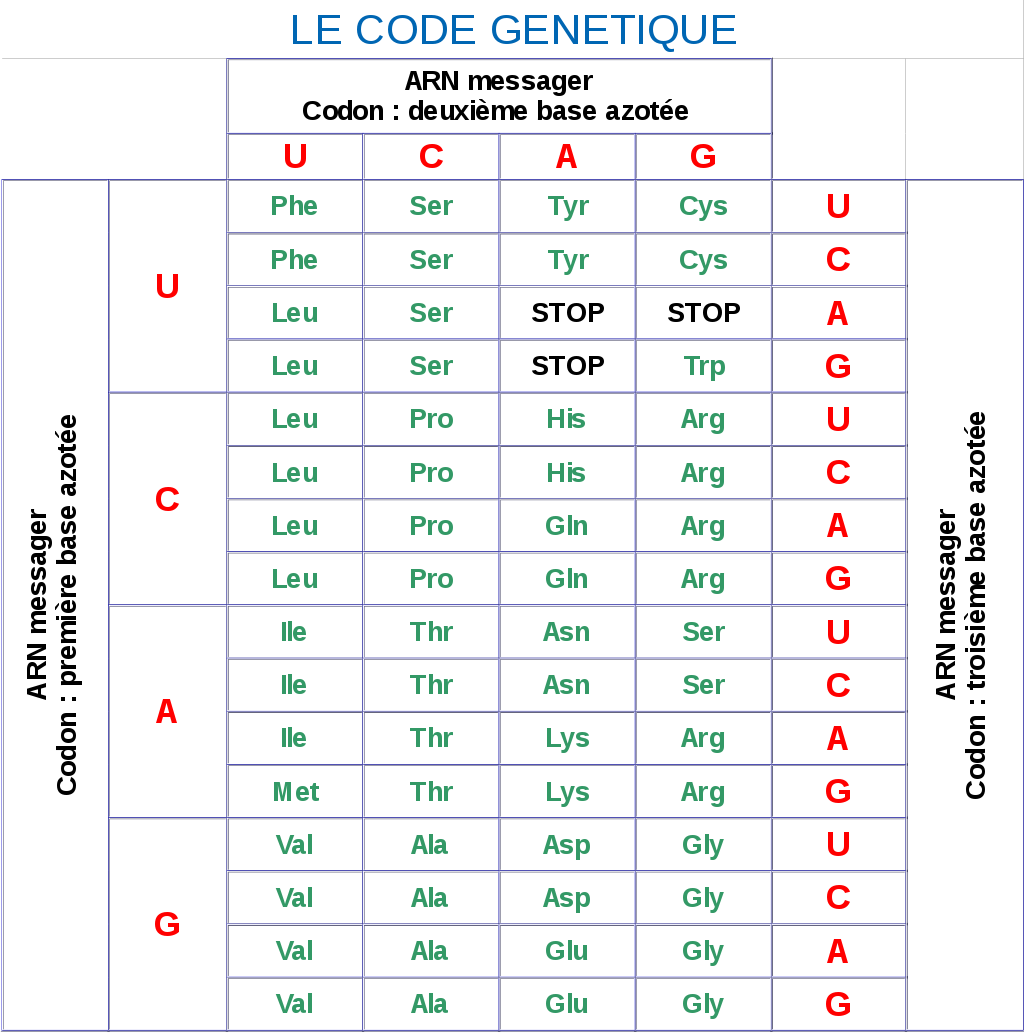
\includegraphics[width=0.95\textwidth]{img/intro/code_genetique.png}
    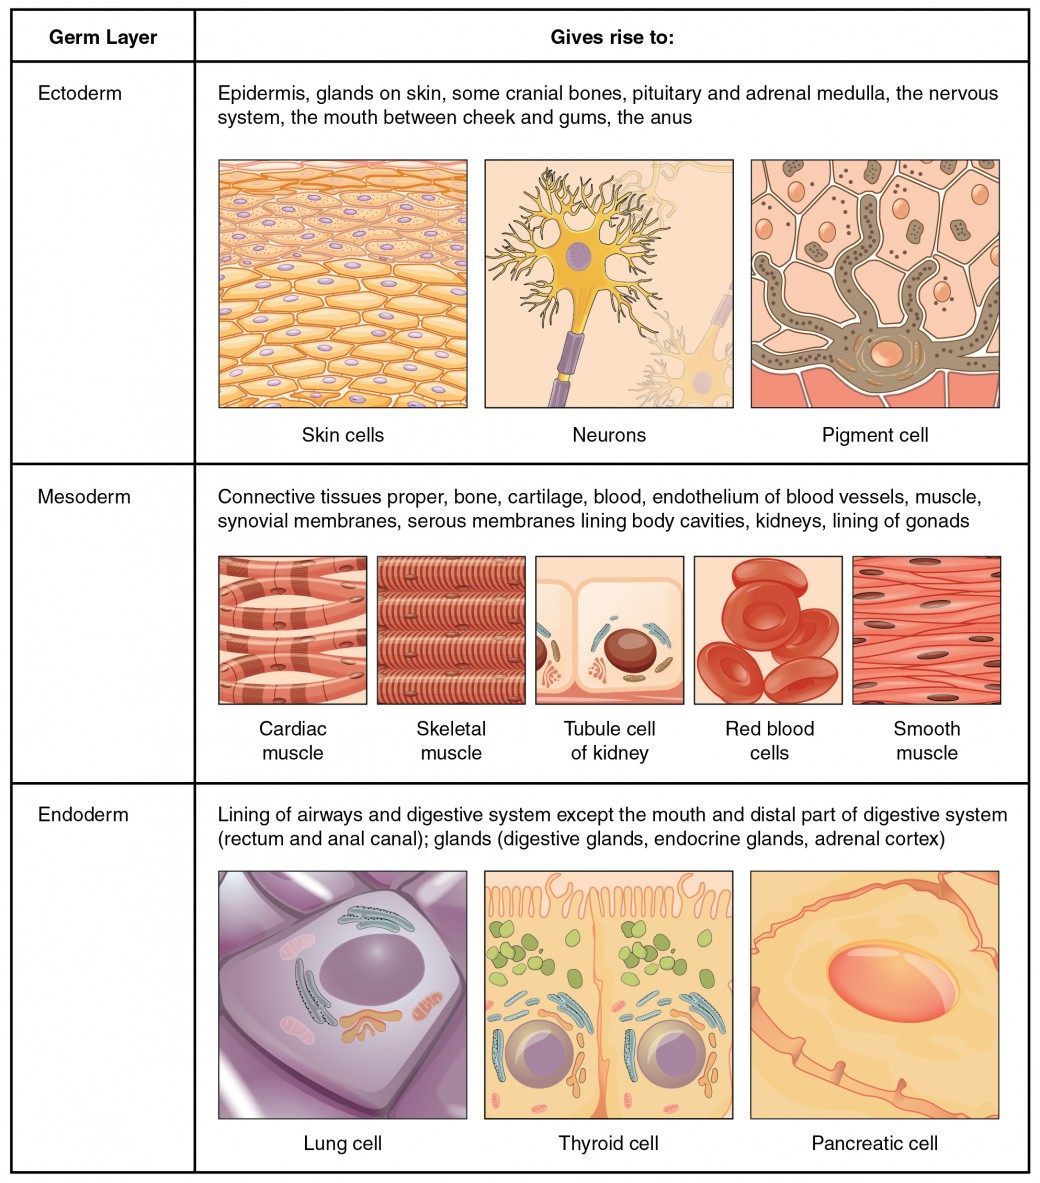
\includegraphics[width=0.8\textwidth]{img/intro/cell_type_feuillet.jpg}
    \caption{Exemple de la diversité de cellules selon le tissu et feuillet embryonnaire dont elles sont issues.}
    \label{fig:intro_tissu_type_cellulaire}
\end{figure*}


Pour effectuer chacune de ces tâches spécialisée, les cellules de type différent vont produire en partie des protéines ayant des fonctions biologiques différentes de ses voisines. La Gene Ontology distingue 32 ontologies (catégories de fonctions) qu'on peut regrouper en 3 familles de fonctions [ISBN 9780138004644]: 
\begin{itemize}
    \item les fonctions catalytiques : les protéines, dans ce cas appelées enzymes, comportent une activité d'augmentation du taux de réaction chimique en diminuant l'énergie d'activation nécessaire. Ces enzymes sont spécifiques d'une transformation d'un substrat vers un produit. Elles peuvent cependant voir leur fonction altérée par des activateurs (co-facteurs, co-enzymes) et des inhibiteurs (co-respresseurs). Ex : la \beta-galactosidase va catalyser la transformation du lactose en glucose + galactose dans l'opéron lactose [10.1016/S0022-2836(61)80072-7].
    \item les fonctions de signalisation/liaison : en se fixant à un recepteur ou en étant un récepteur à la fixation d'un ligand, les proteines permettent de faire transiter de l'information en intra ou extra cellulaire. La fixation entraine la transmission d'un signal physique ou chimique via une cascade d'événements qui vont conduire à une réponse cellulaire. Ex : la production d'une protéine d'insuline par le pancréas va, en se fixant sur les récepteurs membranaires des cellules, déclancher des mécanismes de stockage du glucose. Cela se traduit dans le foie par l'initiation de la transformation du glucose en glycogène.
    \item les fonctions de structuration : les protéines par leur forme et propriétés physico chimiques hautement modulables permettent de donner une architecture et/ou des propriétés mécaniques aux cellules dans/autour desquelles elles se trouvent. Ex : la combinaison de proteines de myosin II et d'actin permettent la contraction musculaire par des phénomènes de coulissage de ces protéines.
\end{itemize}


Pour être produites, ces protéines suivent chacune un plan de construction prédéfini appelé code génétique. Stocké dans une molécule d'ADN (Acide DesoxyRibonucléique) pour chaque chromosome, ce code est présent à l'identique dans chacune des cellules d'un organisme. L'ADN est un polymère de longueur variable selon les espèces et dont la séquence est composée de 4 types de nucléotides : adénosine, tyrosine, guanine, et cytosine. Au long de sa séquence, l'ADN stocke l'information relative aux protéines sous forme d'unités qu'on nomme gène, de telle façon qu'une protéine n'est produisible que par un seul gène. Chez l'homme (sur qui on se concentrera dans ce manuscrit) la version 37 de GENCODE [https://www.gencodegenes.org/human/stats.html] considère ainsi qu'il existe 60 651 gènes. Cependant, tous parmis eux ne produisent pas de protéine. On distingue en réalité les gènes dits "codants" (19951 toujours dans GENCODE 37) car produisant des protéines, et les gènes "non-codants" qui codent pour plusieurs autres entités moléculaires utiles à la cellules.

Chez l'homme et plus généralement les eucaryotes, l'ADN est contenu dans le noyau de la cellule où il se trouve condensé après plusieurs étapes de repliement à l'aide de protéines appelées histones. La machinerie cellulaire de production des protéines étant située à l'extérieur du noyau, une étape intermédiaire de transcription est nécessaire afin de copier la séquence ADN d'un gène sous la forme d'une molécule capable de sortir du noyau : l'ARN messager (ARNm). Semblable à l'ADN, l'ARNm est cependant mono brin alors que l'ADN est double brin (d'où sa représentation classique en échelle), il ne possède pas de thymine mais à la place de l'uranine, et il est évidemment de beaucoup plus petite taille car il n'embarque que l'information correspondant à un gène seulement. Chacun des triplets de nucléotides sur sa séquence encode pour un des 20 types d'acides aminés constituant la protéine associée (Figure \ref{fig:intro_code_genetique}).

\begin{figure*}[!ht]
    \centering
    % 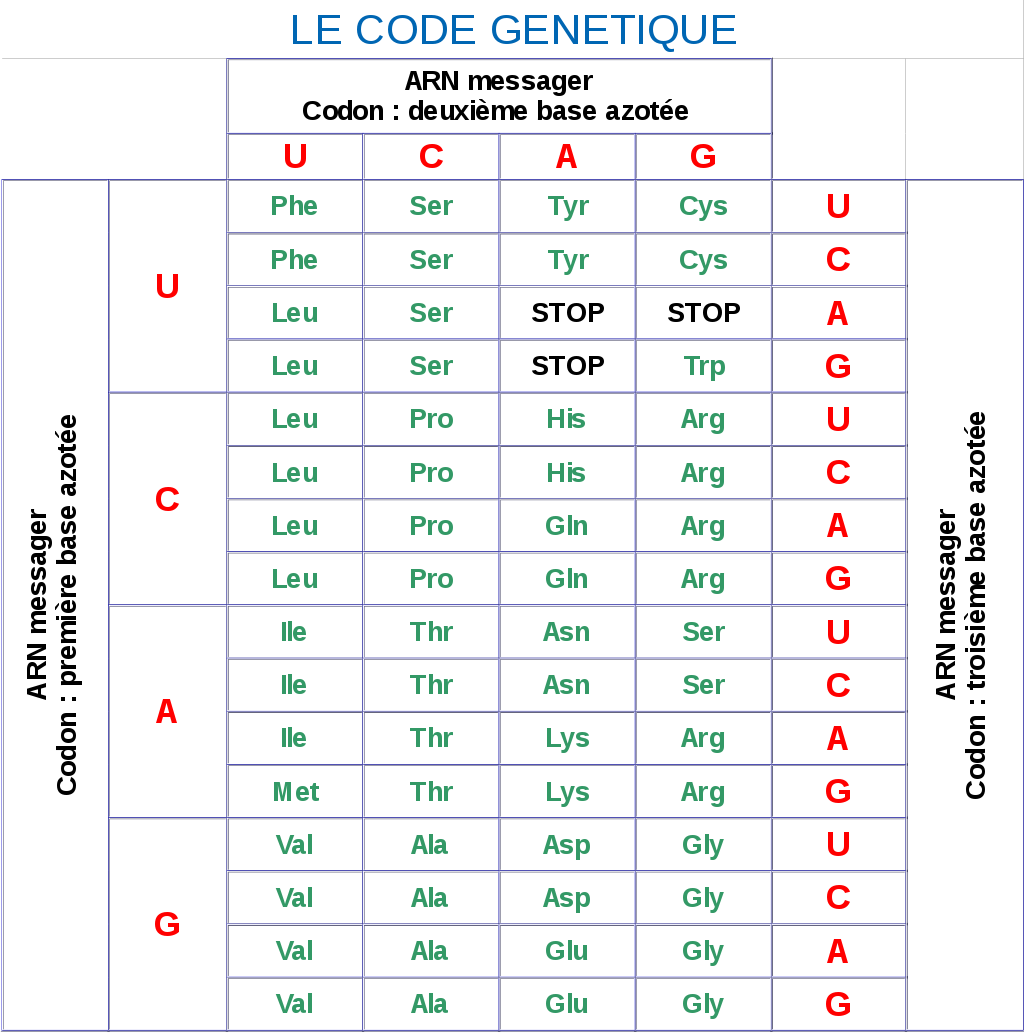
\includegraphics[width=0.95\textwidth]{img/intro/code_genetique.png}
    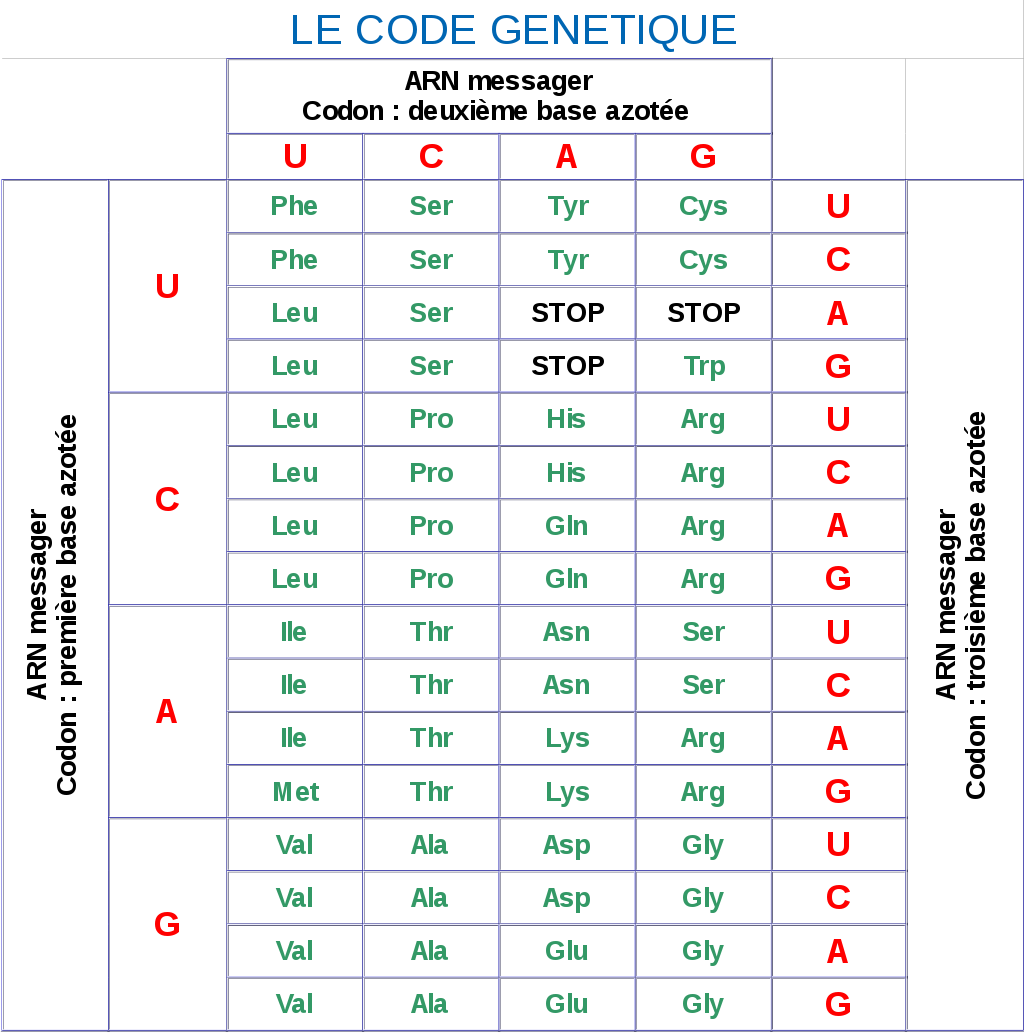
\includegraphics[width=0.8\textwidth]{img/intro/code_genetique.png}
    \caption{Correspondance de triplets de nucléotides avec l'acide aminé produit.}
    \label{fig:intro_code_genetique}
\end{figure*}


Une fois copié depuis l'ADN, l'ARNm immature sort du noyau vers le cytoplasme pour subir une étape de maturation : composé de sous unités appelées introns et exons, l'ARNm se voit retirer ses introns et certaines sections d'exons selon les besoin de sous-fonction de la protéine finale. On nomme "transcrits" toutes ces variations d'ARNm d'un même gène (Figure des modes d'épissage alternatif). Ainsi, on considère que la transcription d'un gène sous n'importe lequel de ses transcrits correspond à l'expression de son gène dans un échantillon. Par la suite, une étape de traduction de l'ARNm en polymère d'acides aminés donnera la base de la protéine. Après un repliement du polymère et des modifictions dites "post-traduction" par la machinerie cellulaire, la protéine sera enfin opérationnelle pour réaliser la fonction qui lui incombe. 


\subsection{La régulation de l'expression pour une spécification cellulaire}

On l'a dit précédemment, l'ADN est identique dans toutes les cellules d'un organisme, alors même que chaque cellule est capable de n'exprimer que les gènes spécifiques à sa fonction (de la myosine pour les myocytes, de la kératine pour les kératinocytes, etc.). Cette capacité ddes cellules est en fait permise par des mécanismes de régulation de l'expression des gènes (et par extension la répression) qui sont établis dès les premières différenciations cellulaire dans le développement d'un organisme. Tout ces mécanismes sont imbriqués pour ajuster au plus fin l'expression des gènes et donc la quantité de la ou les protéines necessaires à l'instant t à la cellule. On distingue les mécanismes suivants : 
\begin{itemize}
    \item \textbf{La régulation de l'initiation de la transcription} : lors de la transcription de l'ADN d'un gène en ARNm, l'ARN polymérase chargée de la transcription vient se fixer sur l'ADN sur le site d'initiation de la transcription (appelé promoteur) pour ensuite commencer à lire la séquence. La fixation au préalable d'une protéine sur ce site (facteur de transcription) entraine alors l'impossibilité de fixation de l'ARN polymérase chargée de la transcription ou à l'inverse favorise son recrutement pour la transcription du gène visé. Très souvents présents dans des boucles de retro-action, ces facteurs de transcription peuvent ainsi être eux-même inactivés par des substances variées. L'exemple le plus connu est l'opéron lactose : en présence de lactose dans la cellule, le facteur de transcription (represseur) lacl est inactivé par la fixation de lactose sur lui même et de la \beta-galactosidase codée par le gène lacZ est produite. En l'absence de lactose, il est libre de se fixer sur le promoteur lac qui est le site d'initiation de la transcription pour les gènes lacZ, lacY, et lacA.
    \item \textbf{La conformation de la chromatine} : les repliements de l'ADN pour la condenser dans une cellule implique de rendre spatialement disponible certaines régions à la transcription et indisponible d'autres.
    \item \textbf{La modification post transciptionnelle} : les ARNm nécessitent l'ajout d'une 7-methylguanosine sur l'extrémité 5' (coiffe 5'), un épissage alternatif, et une polyadenylation (queue poly A) sur l'extrémité 3' afin d'être traduits en protéine. En leur absence, ces ARNm sont détruits par la cellule.
    \item \textbf{La méthylation} : les îlots CpG situés sur l'ADN (notamment dans les promoteurs) peuvent subir l'ajout d'un groupement méthyl, empêchant alors la fixation de différents agents de la transcription.
    \item \textbf{La susceptibilité à la dégradation} : afin de perdurer plus de quelques minutes dans la cellule [Yu2001], certains ARN contiennent ou évitent des motifs de nucléotides influant la vitesse de dégradation (éléments riches en AU, codon stop prématuré, taille de queue poly-A). Des ARN non codants (ARNmi et ARNip) se fixant sur eux peuvent également favoriser leur dégradation.
    \item \textbf{La régulation de la traduction} : le contrôle du recrutement des sous unités des ribosomes, leur altération, ou la compétition des ARN de transfert (ARNt) pour la terminaison sont des paramètres impactant la production finale d'une protéine sans erreur et ne sera donc pas dégradée.
% [Yu2001]: Yu J, Russell JE. Structural and functional analysis of an mRNP complex that mediates the high stability of human beta-globin mRNA. Mol Cell Biol. 2001;21(17):5879-5888. doi:10.1128/mcb.21.17.5879-5888.2001 
\end{itemize}


\#\#\#\#\#\#\#\#\#\#\#\#\#\#\#\#\#\#\#\# FIN DE LA REDACTION PROPRE  \#\#\#\#\#\#\#\#\#\#\#\#\#\#\#\#\#\#\#\#




Lors des perturbation (maladie, stress, âge, etc.) du fonctionnement cellulaire normal, sain, cette régulation de l'expression s'en retrouve pertubée. Le transcriptome (ensemble des ARN ou transcrits produits) est alors un témoin direct des fonctions mises en défaut. L'étude de la quantité de chacun donne ainsi un moyen direct direct de comprendre l'origine d'effets macroscopiques (irritation atopique, tumeur, nécrose, etc.) ou moléculaires (augmentation du taux de glucose, malabsorption de nutriments, augmentation du pH, etc.).

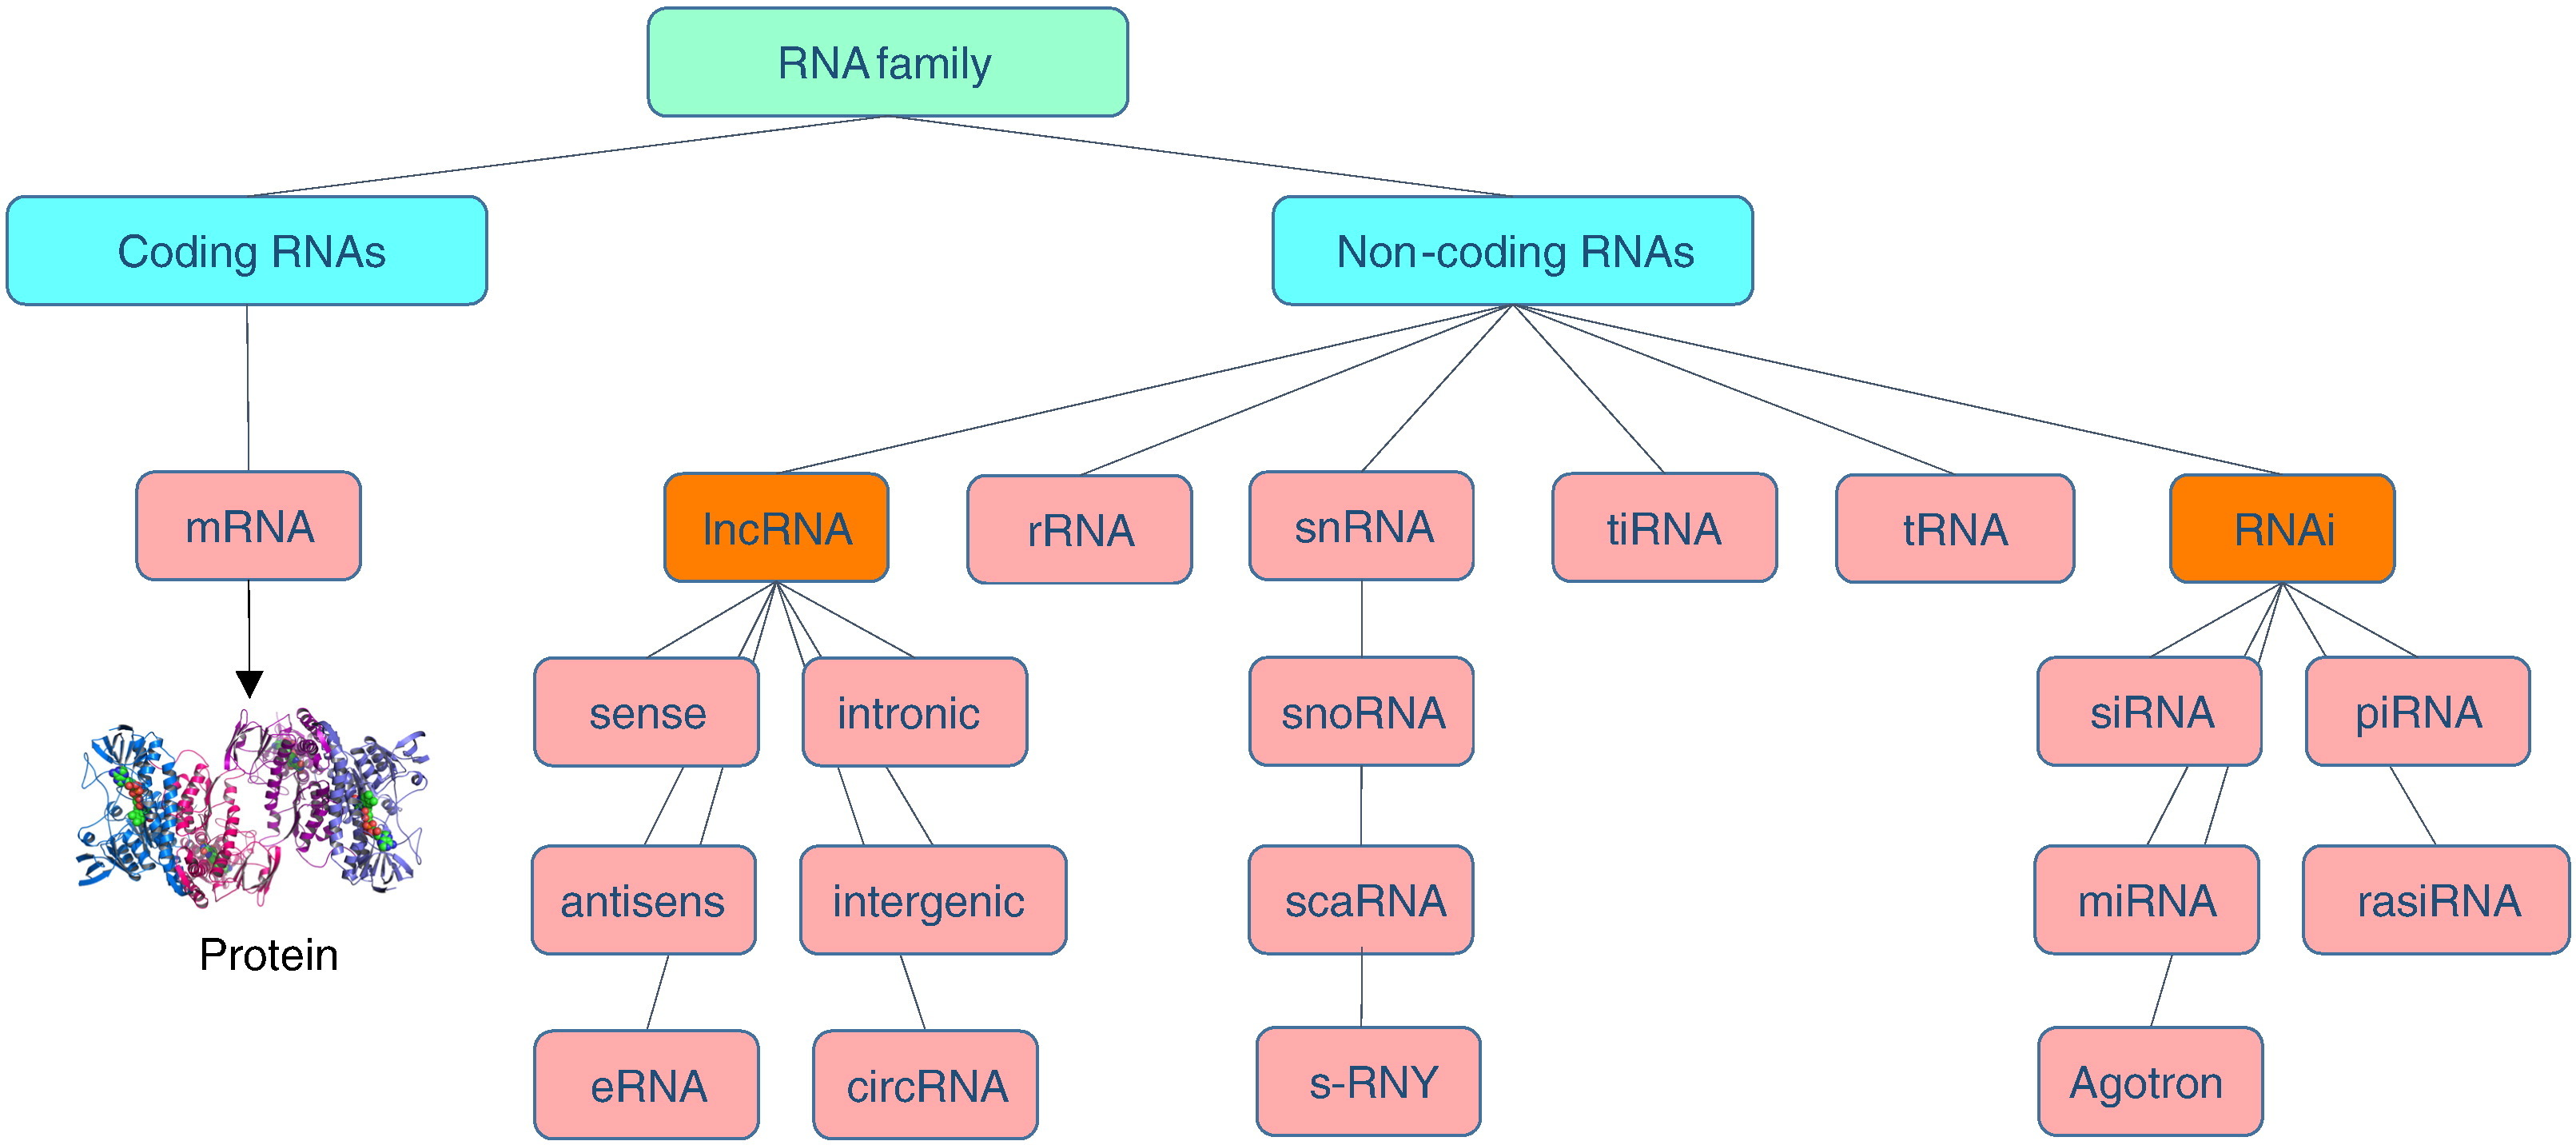
\includegraphics{img/intro/rna_familly_tree.jpg}
%% https://www.sciencedirect.com/science/article/pii/S0167488916302919

%% TRANSITION : parler des erreurs/variabilité biologique ? 

% \subsection{L'étude des perturbation du vivant pour la résolution de conditions cliniques}
\subsection{L'étude des perturbation de l'expression pour la résolution de conditions cliniques}

\section{Les technologies de séquençage de l'expression des gènes}
%% TODO : merge avec 1.1 partie d'avant

%% Nb publi pour le ration de microarray / RNA seq de jeux de données ?


%% historique des techno et qques specificités : https://journals.plos.org/ploscompbiol/article?id=10.1371/journal.pcbi.1005457
\begin{itemize}
\item Avant propos sur le développement des technologies de séquençage avec la quantification d'ARNm par rt-qPCR, le séquençage par gel, etc.
\item Transition vers les technologies de séquençage nouvelle génération
\item Expliquer qu'actuellement ce ne sont quasiment plus que le microarray et le RNA-seq qui sont utilisé (= transition expliquant pourquoi on ne détaille qu'eux par la suite)
\end{itemize}

%% Un TRES bon site sur les technos de sequencage : http://education.knoweng.org/sequenceng/



\subsection{Microarray}

\subsubsection{But et protocole}

Principe de la puce à ADN/ARN
Coloration mono/duo
Préparation de librairie
Construction des puces
Exemples d'utilisation ?

\subsubsection{Propriétés mathématiques/techniques et normalisation}
\label{subsubsection:microarray_props_and_normalisation}

Distribution
\begin{itemize}
\item  "Données continues, il est possible de construire des modèles d’analyse statistique ense basant sur des hypothèses de normalité des données (Smyth, 2004). Ces techniquesd’analyse, adaptées aux données gaussiennes ne peuvent pas être appliquées directementaux données RNA-seq qui sont des données de comptage, discrètes et positives" %% https://tel.archives-ouvertes.fr/tel-01424124/document
\item     Normalisation : Normalization is a process designed to identify and correct
\item technical biases. 2 types of norm : Between and within normalization (cf. formation marie laure meme si c'est pour le RNA-seq). Pourquoi normalisation log2 : le log pour passer à une échelle symétrique autour de 0, le 2 car c'est + facile à interpréter, chaque fois qu'on augmente le ratio Ti de 1, on double la up regulation  
\end{itemize}
%%(https://www.researchgate.net/post/Why_do_we_usually_use_Log2_when_normalizing_the_expression_of_genes et https://www.nature.com/articles/ng1032z)
Contrôle qualité
Filtration ?


Explication du déclin au profit du RNA-seq mais avec contraste sur son utilité quand pas besoin de whole transcriptome.



%% INFOS ET FORMULATION SUR LA NORMALISATION
% Parmi les biais biologiques classiques, on retrouve le contenu en GC, la longueur des transcrits, la quantité d'ARN total,  weighted linear regression (lowess).
% Pour corriger ces biais biologiques, plusieurs méthodes ont été proposées prenant chacune plus ou moins de biais en compte  : 
% linear regression analysis1, log cen- tering, rank invariant methods2 and Chen’s ratio statistics3
% SOURCE : 10.1038/ng1032


\subsection{RNA-Seq}

\subsubsection{But et protocole}

Principe
\begin{itemize}
\item Un mot sur le fait qu'on applique pas les mêmes méthodes de normalisation car la nature du signal n'est pas le même : une fluorescence pour le microarray (variable continue), et un comptage dans le cas du RNA-seq (variable discrète).
\item Explication de l'essor du RNA-seq (couts, precision, etc.)
\end{itemize}

\subsubsection{Propriétés mathématiques/techniques et normalisation}
\label{subsubsection:rnaseq_props_and_normalisation}

Distribution(binomiale negative) %% Justification binomiale negative "Negative binomial (NB) distribution is the established gold standard, because of its ability to accurately model RNA-seq data with a low number of available replicates [7]." https://doi.org/10.1093/bib/bbx115
Normalisations%% cf. formation marie laure, il y a toutes les refs de publi a prendre
%% La raison du l'utilisation des pseudo counts et du log dans le RNA-seqyo : https://www.biorxiv.org/content/biorxiv/early/2020/05/19/2020.05.19.100214.full.pdf
\begin{itemize}
    \item Within sample
    \item Between samples
\end{itemize}
%% À classer entre within/between plus ahut selon ce qui est marqué dans la formation de marie laure : taille de librairie (= profondeur de sequencage), contenu en GC, taille des gènes, composition de la population d'ARN de chaque condition), contrôle qualité, filtration  (https://www.biostars.org/p/349881/)



%%%%%%%%%%%%%% LE TRAITEMENT STATISTIQUE DE L'INFORMATION BIOLOGIQUE %%%%%%%%%%%%%%


\section{Le traitement statistique de l'information biologique}
\subsection{L'expression différentielle : les acteurs majeurs}
\begin{itemize}
  \item Méthode de capture des acteurs majeurs
  \item Pas d'étude du système 
% \item Des statistiques descriptives à l'expression différentielle %% Bof, j'ai pas retrouvé de stade "stats explo" 
\end{itemize}

\subsection{La modélisation du vivant : des acteurs au système}
\begin{itemize}
\item De la régulation des gènes à son approximation par des modèles statistiques, en passant par la biologie des systemes qui est trop couteuse pour des organismes complexes %% mal formulé car dans le desordre (le dernier point devrait venir en 2e)
\item Transistion vers la modélisation par encodage de l'information dans des réseaux qui sont en fait des graph et qui sont moins couteux car probabilistes (ils ne sont pas la vérité mais une approximation)
\end{itemize}

\subsection{Les réseaux biologiques : le système vu via la théorie des graphes}
\begin{itemize}
\item Principe : les graphes sont une méthode de plus en plus utilisée dans la représentation du fonctionnement d'organismes puisqu'ils permettent d'avoir une vision à l'échelle du système tout entier.
%% Jolie intro à s'inspire : https://www.nature.com/articles/s41467-019-08746-5
\item Différences / ressemblance entre graphe et reseau ?
\item Les types de réseaux/graphes rencontrés en biologie et plus particulièrement en expression des gènes : small-world
\item Les problèmes de visualisation de grands réseaux %% section layout de ce livre https://sites.fas.harvard.edu/~airoldi/pub/books/BookDraft-CsardiNepuszAiroldi2016.pdf
\end{itemize}


%%%%%%%%%%%%%%%%%% LES RESEAUX DE CO-EXPRESSION %%%%%%%%%%%%%%%%%%


\section{Les réseaux de  co-expression}

%% GROOOOOSSSE PUBLI REVIEW sur la co-expression ET la comparaison de modules, aka co-expr differentielle https://doi.org/10.1109/TCBB.2019.2893170

\subsection{But}
"Gene co-expression networks seek to identify transcrip- tional patterns indicative of functional interactions and regulatory relationships between genes" %%https://genomebiology.biomedcentral.com/articles/10.1186/s13059-019-1700-9 + Barabási A-L, Gulbahce N, Loscalzo J. Network medicine: a network-based approach to human disease. Nat Rev Genet. 2011;12:56–68. + Furlong LI. Human diseases through the lens of network biology. Trends Genet. 2013;29:150–9.

\subsection{Principe}
%% Relire `van Dam, S., Võsa, U., van der Graaf, A., Franke, L. & de Magalhães, J. P. Gene co-expression analysis for functional classification and gene–disease predictions. Brief. Bioinform. bbw139 (2017). doi:10.1093/bib/bbw139`
\begin{itemize}
    \item Réseaux binaires (0 = pas de connexion, 1 = connexion). Pour et contres.
    \item Réseaux pondérés. Pourquoi c'est vers ça qu'on s'est orientés ? Car les connections entre gènes ne sont pas binaires, elles sont plutot multiples et très dépendantes temporellement. Une meme cellule échantillonnée à des temps différents aura un profil plus ou moins différent. On y retrouvera les grandes fonctions clefs mais les aspects plus variables auront peut etre changé. D'où aussi la nécessité d'un bon nombre d'échantillons pour assurer la validité des résultats. Sinon les correlations ne sont pas représentatives.
\end{itemize}

\subsection{Construction}
\begin{itemize}
\item Pourquoi utiliser les counts plutôt que les FPKM, TPM, etc.
\item Quelles étapes de pré-traitement ?
\item Les différents scores de similarité : Pearson, Spearman, bicor, mutual information
\item La pondération des scores (adjacence et TOM) et la propriété d'invariance d'échelle (scale-free). Reparler de barbarasi et son celebre article (https://science.sciencemag.org/content/325/5939/412/tab-pdf) + Pourquoi elle est parfois encore discutée (https://www.nature.com/articles/s41467-019-08746-5) alors que tout de même pertinente en biologie. 
\end{itemize}
\subsection{Détection de modules}
\begin{itemize}
    \item Notion de communauté
    \item Définition du partitionnement (clustering) et des différentes techniques
\end{itemize}

\subsection{Exploitation des modules de gènes}

\subsubsection{Intégration biologique}
%% AKA knowledge driven
\begin{itemize}
    \item Enrichissement
    \item Test d'association
\end{itemize}

\subsubsection{Association phenotypique}
%% aussi knowledge driven

%%\subsection{Capitalisation sur l'information intrinsèque aux données}

\subsubsection{Étude topologique}
%% AKA data driven

%% Note : à voir si je présente aussi ici la comparaison de module vu que je vais ptet évoquer l'expression differentielle ici pour faire le parallele avec l'analyse transcripto classique. Sinon ça ira dans l'intro du chapitre avec l'article de GWENA.

\begin{itemize}
    \item Degré
    \item Définition de hub gene
    A trier / ordonner entre les différentes définitions, ce qu'elles visent, ce qu'elles appaortent et si possible une comparaison d'entre elles. On distinguera les mesure purement basées sur la theorie des graphs et celles impliquant des mesures statistique de significativité d'un gene comme hub (cf publi sur DHGA)
    \begin{itemize}
        \item Def 1 : Network theory : "A node is defined as hub node, if its connection degree is greater than average connection degree of the network" %% https://www.ncbi.nlm.nih.gov/pmc/articles/PMC5215982/
        \item Def 2 : Network hubs, the core elements in the network, can be defined using a range of different measures. These measures quantify distinct aspects of topological centrality, which can be defined as the capacity of a node to influence or be influenced by other nodes by virtue of its connection topology (Fornito et al., 2016).
    \end{itemize}
\end{itemize}
\subsubsection{Expression différentielle}
Pas sur de foutre ca là... Peut etre plutot en intro de la section complete en guise de "En analyse RNA classique, une méthode data driven est l'expression différentielle, mais en co-expression on a a disposition plus d'information extractable, et ce grace a la theorie des graphes" 

\subsubsection{Comparaison de modules}

Ou co-expression différentielle
%% "However, searching for differences in networks requires great sensitivity to the initial choice of data. For example, the absence of a shared link in mouse and human co-expression networks does not necessarily indicate divergent function. Instead, differences in the mouse and human co-expression networks may indicate differences in the technical platforms or the experimental conditions used to build the networks" http://doi.org/10.1371/journal.pgen.1000776

\subsection{Interprétation des résultats}

\subsubsection{Comparabilité des résultats issus de RNA-seq et de microarray}
\begin{itemize}
    \item Pas les meme hub genes %% "Microarray and RNA-seq-derived networks have different hub genes" https://academic.oup.com/bioinformatics/article/31/13/2123/196230
\end{itemize}


%%%%%%% L'INTÉRÊT DE l'ANALYSE PAR CO-EXPRESSION POUR L'ÉTUDE DU VIEILLISSEMENT %%%%%%%


\section{Le vieillissement, système hautement imbriqué}
%% Idée de début de paragraphe
S'il est une condition biologique où les réseaux de co-expression sont particulièrement bien adpatés, c'est bien le vieillissement. Source multi-factorielle de changements dans l'organisme, il est chez l'humain à l'origine d'une dégradation progressive des fonctions de base du corps.

% Aide à la justification de l'utilisation de la co-expression dans l'étude du vieillissement : 10.1016/j.arr.2009.10.006

%% GROSSE REVIEW : 10.1007/978-3-030-25650-0

\subsection{Définition biologique}

%% Liens utiles :
% https://www.nature.com/articles/35041709
% https://www.nature.com/articles/nrm.2017.68 maladies définies comme associées à l'âge
% ACcumulation erreurs et lien avec la mortalité (page 123) https://www.sciencedirect.com/science/article/abs/pii/S095506741730131X
% Age dependant/independant mortality : https://en.wikipedia.org/wiki/Gompertz%E2%80%93Makeham_law_of_mortality
% REview biomarqueurs et forces d'action sur le vieillissement : https://sci-hub.se/10.1007/978-3-030-25650-0

% "Two evolutionary theories of ageing — the mutation-accumulation and trade-off theories "


%% À reformuler comme définition du vieillissement mais le contenu est sympa
% Aging is the inevitable time-dependent decline in physiological organ function and is a major risk factor for cancer development. Due to advances in health care, hygiene control and food availability, life expectancy is increasing and the population in most developed countries is shifting to an increasing proportion of people at a cancer susceptible age.

\begin{itemize}
    \item Phenomène à la fois génétique (intrinseque) [] et environemental (extrinseque) 
    \item Facteurs (hallmarks) : raccourcissement des télomères, phénomènes d'inflammation, réduction de la machinerie cellulaire
    % Sterile inflammation, also known as ‘inflammaging’, is a hallmark of ageing and a contributing factor to many age-related diseases ( https://doi.org/10.1093/gerona/glu057). 
    \item Manifestation : Ralentissement de la division cellulaire, développement de cellules non-fonctionnelles / nocives (aka tumeurs), malfonctionnement des tissus/organes
    \item Le vieillissement, contrairement aux maladies mendéliennes, est multifactoriel est se manifeste donc sous la forme d'un spectre
    \item Différence Âge chronologique / âge biologique
    \item Différence vieillissement (aging), longévité (longevity/lifespan), survie en bonne santé (health-span) 
\end{itemize}

\textbf{Bouts de textes récupérés de l'intro du chap2 car mieux ici}

Il se manifeste dans chacun sous des formes  différente avec pour certains
Une difficulté supplémentaire se présente alors lors de l'isolement de biomarqueurs : les changements biologiques entraînés par l'altération de ces biomarqueurs lors du vieillissement sont-ils 
entraînés par des mécanismes distincts au sain du tissu considéré ou bien sont-ils communs entre plusieurs changements et/ou tissus ?
% un phénomène local au tissu ou bien plus général avec une incidence dans le tissu considéré ?
% Sont-ils la cause ou la conséquence du vieillissement. 
Une même modification avec le temps telle que le raccourcissement des télomères (abordé en X.X.X\todo{ref intro vieillissement}) peut ainsi donner des affections variable selon le tissu : fibroses pulmonaires, des anémies aplasique, des dyskératoses congénitale, etc. \cite{Armanios2012} (Table \ref{table:tissu_telomere_effet}). 

\begin{table}[h]
\resizebox{\textwidth}{!}{
\begin{tabular}{m{0.2\textwidth}m{0.2\textwidth}m{0.6\textwidth}}
\textbf{Type de tissu}                                                                    & \textbf{Nom du tissu}                                            & \textbf{\begin{tabular}[c]{@{}l@{}}Manifestations pathologiques chez l'humain \\ avec syndromes télomériques\end{tabular}} \\ \hline
\multirow{4}{*}{\begin{tabular}[c]{@{}l@{}}Tissus à fort\\ renouvellement\end{tabular}}   & Peau                                                             & • Blanchissement prématuré des cheveux                                                                                     \\
                                                                                          & \begin{tabular}[c]{@{}l@{}}Moelle \\ osseuse\end{tabular}        & • Anémie aplastique                                                                                                        \\
                                                                                          & Immune                                                           & \begin{tabular}[c]{@{}l@{}}• Infections opportuniste\\ • Immunodéfiscience des cellules B, T et NK\end{tabular}            \\
                                                                                          & \begin{tabular}[c]{@{}l@{}}Épithélium \\ intestinal\end{tabular} & \begin{tabular}[c]{@{}l@{}}• Entérocolite\\ • Émoussement villositaire\end{tabular}                                        \\
\multirow{3}{*}{\begin{tabular}[c]{@{}l@{}}Tissus à faible\\ renouvellement\end{tabular}} & Poumon                                                           & \begin{tabular}[c]{@{}l@{}}• Emphysème prématuré\\ • Fibrose pulmonaire idiopathique\end{tabular}                          \\
                                                                                          & Foie                                                             & • Fibrose-cirrhose du foie cryptogénétique                                                                                 \\
                                                                                          & Os                                                               & \begin{tabular}[c]{@{}l@{}}• Ostéoporose\\ • Nécrose avasculaire\end{tabular}                                              \\
Cancer                                                                                    & Multi-tissus                                                     & \begin{tabular}[c]{@{}l@{}}• Cancers épithéliaux\\ • Hémopathies malignes\end{tabular}                                    
\end{tabular}
}
\caption{Phénotypes de maladies spécifiques aux organes chez les humains ayant des télomères courts. Modifié d'après la Table 2 de Armanios 2012, \textit{The telomere syndromes} \cite{Armanios2012}}
\label{table:tissu_telomere_effet}
\end{table}



\subsection{Enjeux}

% Le vieillissement est un phénomène à distinguer de la longévité qui ne tient pas compte de l'aspect dégradation de la santé. 

% Si la quête pour l'immortalité n'est pas souhaitable pour plusieurs raisons tant éthiques qu'économiques \cite{Hayflick2000}, la recherche pour un vieillissement en bonne santé se doit-elle de continuer.

De Magalhães s'interrogeait en 2003 \cite{deMagalhes2003} d'une programmation génétique du vieillissement. La question sous-jacente abordée était finalement de savoir si analyser et comprendre indépendemment chaque conséquence néfaste et maladie apparaissant avec l'âge n'était pas une course perdue d'avance pour les combattre. Ainsi, De Magalhães envisageait que comprendre le fonctionnement global du vieillissement serait plus pérenne pour retarder d'un seul coup l'apparition de quelques, si ce n'est toutes, maladies chez la personne âgée.

Le vieillissement est donc, part les pathologies qu'il entraîne, un enjeu de santé publique.


\begin{itemize}
    \item Susceptibilité aux maladies opportunistes
    \item tdeetAutonomie patient
    \item Médicalisation précoce
\end{itemize}

\subsection{La capture de l'information liée au vieillissement par la transcriptomique}
\label{}

\begin{itemize}
    \item La dérégulation de la transcription comme phénomène précédemment mentionné
    \item L'analyse d'expression différentielle + d'autres analyses discrètes (au sens de Barabasi) ont permis d'isoler plusieurs gènes associés à un ou plusieurs tissu vieillissant. \label{intro_biomarker_aging}
    \item la création de bases de données liées au vieillissement sous toutes ses formes : gènes associés au vieillissement dans différents tissus et chez différentes espèces modèle, signatures de scenescence, gènes associés au ralentissement du vieillissement par restriction calorique, médicaments anti vieillissement, gènes associés à la longévité, changements liés au vieillissement à différents niveaux (biological levels, integrating molecular, physiological and pathological age-relate). En gros tout https://genomics.senescence.info/
    \item L'insuffisance de la capture de biomarqueurs pour un processus aussi compliqué que le vieillissement. Donc la nécessité d'une étude en réseau
    \item 
    
\end{itemize}
%% https://doi.org/10.1007/978-981-32-9005-1_3
%% https://www.sciencedirect.com/science/article/abs/pii/S0959438820300878
%% https://onlinelibrary.wiley.com/doi/abs/10.1111/acel.13280

\section*{Phrases utiles à retravailler et intégrer}

\begin{itemize}
\item "Studies have shown that each gene is estimated on average to interact with four to eight other genes1 and to be involved in 10 biological functions" [10.1038/s41598-017-18705-z]
\item "A very clear partition of different biological networks is provided by Christensen et al. [1], who separated these networks into five main categories as follows: [metabolic networks, signal transduction networks,transcriptional regulatory networks, protein-protein networks, functional gene networks]" [10.1093/bfgp/elt003]
%% Bouquin à la coloc de Clément à Sète, pas retrouvé sur le net jusque là 
\item "Le vieillissement est un continuum conduisant une personne en bonne santé à une réduction de sa réserve fonctionnelle, puis de sa capacité fonctionnelle et de sa qualité de vie. CEs différents aspects ne décrivent pas un chemin linéaire ou ordonné." [Patient agé : particularités de la consultation, Gilles Berrut]
\item "It has been reported that nearly one in four studies uses public data to address a biological problem without generating new raw data (Rung and Brazma, 2013)." [10.3389/fpls.2016.00444]
\end{itemize}


%% Points que je veux aborder :
%%  - Definition des reseau arrete / noeud
%%  - Definition des modules par l'effet de modularité
%%  - Ce à quoi ils peuvent servir : raccrochage de fonction a certains genes, detection de pathways, detection de reseaux de regulation



%%    • Weighted aspect [trop general, aura plutot sa place dans la thèse]
%% But because of the multi-functionality aspect of each gene, such GCN using only binary state between genes (1 = correlated, 0 = not correlated) lead to information loss\cite{Langfelder2008}. Therefore, a new class of GCN have been developed: weighted gene co-expression networks. One of the most famous implementation is the R package WGCNA\cite{Langfelder2008}, but one can also mention the recent wTO\cite{Gysi2018} package which consider both positive and negative correlation for GCN building. Instead of a simple pairwise correlation, these packages weight the similarity score by calculating a factor taking into account other properties of the network. In the case of WGCNA, it specifies an adjacency score which raise the similarity to a power, which will increase the strength of strong similarities while keeping low week ones. In the case of wTO, it determine an average accounting for all common neighbors of a node.

%%    • Topological aspect
%%    • Co-expression properties (Scale-free-network entre autres ?)



%% Infos sur la peau : these super interessante => https://dumas.ccsd.cnrs.fr/dumas-01599807/document% \end{itemize}

